\documentclass[11pt]{article}




\usepackage[sfdefault]{FiraSans} %% option 'sfdefault' activates Fira Sans as the default text font
\usepackage[T1]{fontenc}
\renewcommand*\oldstylenums[1]{{\firaoldstyle #1}}

\usepackage{natbib}
\usepackage[french,english]{babel}
\usepackage{numprint}
\usepackage{multirow}
\usepackage{rotating}
\usepackage{fancyhdr}
\usepackage{booktabs}
\usepackage{multicol}
\usepackage{hyperref}\hypersetup{colorlinks=true}

\usepackage{amsmath,amssymb,amsfonts,textcomp}
\usepackage{color}
\usepackage{calc}
 \setlength{\tabcolsep}{8pt}
\usepackage{setspace}
\onehalfspacing
\usepackage{longtable}
\usepackage{graphicx}
\usepackage[margin=1in]{geometry}
\setlength{\parindent}{0pt}
\usepackage[bottom]{footmisc}
\pagestyle{fancy}
\usepackage{titlesec}
\usepackage{lipsum}
\usepackage{cancel}
\usepackage{multicol}

\usepackage{amsmath,amssymb}
\usepackage{lmodern}
\usepackage{iftex}
\ifPDFTeX
  \usepackage[T1]{fontenc}
  \usepackage[utf8]{inputenc}
  \usepackage{textcomp} % provide euro and other symbols
\else % if luatex or xetex
  \usepackage{unicode-math}
  \defaultfontfeatures{Scale=MatchLowercase}
  \defaultfontfeatures[\rmfamily]{Ligatures=TeX,Scale=1}
\fi

\titleformat{\section}
  {\normalfont\Large\scshape\bfseries}{\thesection}{1em}{}
  \titlespacing{\section}{0pt}{10pt}{0pt}
\titleformat{\subsection}
  {\normalfont\bfseries}{\thesection}{1em}{}
  \titlespacing{\subsection}{0pt}{6pt}{0pt}
\providecommand{\tightlist}{%
  \setlength{\itemsep}{0pt}\setlength{\parskip}{0pt}}\newenvironment{itemize*}%

  
\lhead{EC200 - Econometrics and Applications}
\rhead{Version: \today}
\setlength\parskip{0.10in}
\begin{document}
\thispagestyle{plain}
\singlespacing


Version: \today \hfill Fall 2021\\
EC200: Econometrics and Applications
%\vspace{1.5cm}
\begin{center}
\Large{\textbf{Problem Set 3}}\\
\end{center}
\bigskip


%{
%\setcounter{tocdepth}{3}
%\tableofcontents
%}


\hypertarget{welcome}{%
\section*{Welcome}\label{welcome}}

We've been so busy with labs and research ideas that we have
\emph{three} chapters of coverage to work through! Note that this is
your last problem set before the next exam

You can download the data file you need for question 6
\href{https://ec200f21.netlify.app/assignment/materials/growth.dta}{here}, along with information on the
variable definitions
\href{https://www.princeton.edu/~mwatson/Stock-Watson_3u/Students/EE_Datasets/Growth_Description.pdf}{here}

\hypertarget{what-do-i-submit}{%
\section*{What do I submit?}\label{what-do-i-submit}}

\begin{itemize}
\tightlist
\item
  Your written up answers to exercise questions. If you work on a piece
  of paper, please scan using some sort of phone software (like
  Microsoft Lens or Adobe Scan) rather than just taking a picture.
\item
  A do-file that runs your Stata analysis (for question 4).
\item
  A log file that includes the output from running your do-file (for
  question 4).
\end{itemize}

\hypertarget{exercises}{%
\section*{Exercises}\label{exercises}}

\begin{enumerate}
\def\labelenumi{\arabic{enumi}.}
\tightlist
\item
  Suppose that we want to estimate the effects of alcohol consumption
  (\(alcohol\)) on college grade point average (\(colGPA\)). In addition
  to collecting information on alcohol consumption and grade point
  averages, we also obtain attendance information (say, percentage of
  lectures attended, \(attend\)). A standardized test score (say,
  \(SAT\)) and high school GPA (\(hsGPA\)) are also available.

  \begin{enumerate}
  \def\labelenumii{\alph{enumii}.}
  \tightlist
  \item
    Should we include \(attend\) along with alcohol as explanatory
    variables in a multiple regression model? What would be the
    interpretation of \(\beta_{alcohol}\) if we did?
  \item
    Should \(SAT\) and \(hsGPA\) be included as explanatory variables?
    Explain.
  \end{enumerate}
\item
  A research plans to study the casual effect of police on crime, using
  data from a random sample of U.S. counties. She plans to regress the
  county's crime rate on the (per capita) size of the county's police
  force.

  \begin{enumerate}
  \def\labelenumii{\alph{enumii}.}
  \item
    Explain why this regression is likely to suffer from omitted
    variable bias. Which variables would you add to the regression to
    control for important omitted variables?
  \item
    Use your answer to (a) and the expression for omitted variable bias
    (from the slides or textbook) to determine whether the regression
    will likely over- or underestimate the effect of police on the crime
    rate. (That is, is \(\hat{\beta_1}>\beta_1\), or that
    \(\hat{\beta_1} < \beta_1\)?)
  \end{enumerate}
\end{enumerate}

\begin{enumerate}
\def\labelenumi{\arabic{enumi}.}
\setcounter{enumi}{2}
\item
  Critique each of the following proposed research plans. Your critique
  should explain any problems with the proposed research and describe
  how the research plan might be improved. Include discussion of any
  additional data that needs to be collected, and the appropriate
  statistical techniques for analyzing those data.

  \begin{enumerate}
  \def\labelenumii{\alph{enumii}.}
  \tightlist
  \item
    A researcher is interested in determining whether a large aerospace
    firm is guilty of gender bias in setting wages. To determine
    potential bias, the researcher collects salary and gender
    information for all of the firm's engineers. The researcher then
    plans to conduct a ``difference in means'' test to determine whether
    the average salary for women is significantly less than the average
    salary for men
  \item
    A researcher is interested in determining whether time in prison has
    a permanent effect on a person's wage rate. He collects data on a
    random sample of people who have been out of prison for at least 15
    years. He collects similar data on a random sample of people who
    have never served time in prison. The data set includes information
    on each person's current wage, education, age, ethnicity, gender,
    tenure (time in current job), occupation, and union status, as well
    as whether the person has ever been incarcerated. The researcher
    plans to estimated the effect of incarceration on wages by
    regressing wages on an indicator variable for incarceration,
    including in the regression the other potential determinants of
    wages such as education, tenure, union status, and so on.
  \end{enumerate}
\item
  Consider a dataset that contains information on 4700 full-time
  full-year workers. The highest educational achievement for each worker
  was either a high school diploma or a bachelor's degree. The worker's
  ages ranged from 25 to 45 years. The data set also contains
  information on the region of the country where the person lived,
  marital status, and number of children. See below for variable
  definitions.

  \begin{enumerate}
  \def\labelenumii{\alph{enumii}.}
  \tightlist
  \item
    Is the college-high school earnings difference estimated from this
    regression statistically significant at the 5\% level? Construct a
    95\% confidence interval of the difference.
  \item
    Do there appear to be important regional differences in hourly
    wearnings? Use an appropriate hypothesis test to explain your
    answer.
  \end{enumerate}
\end{enumerate}
\centering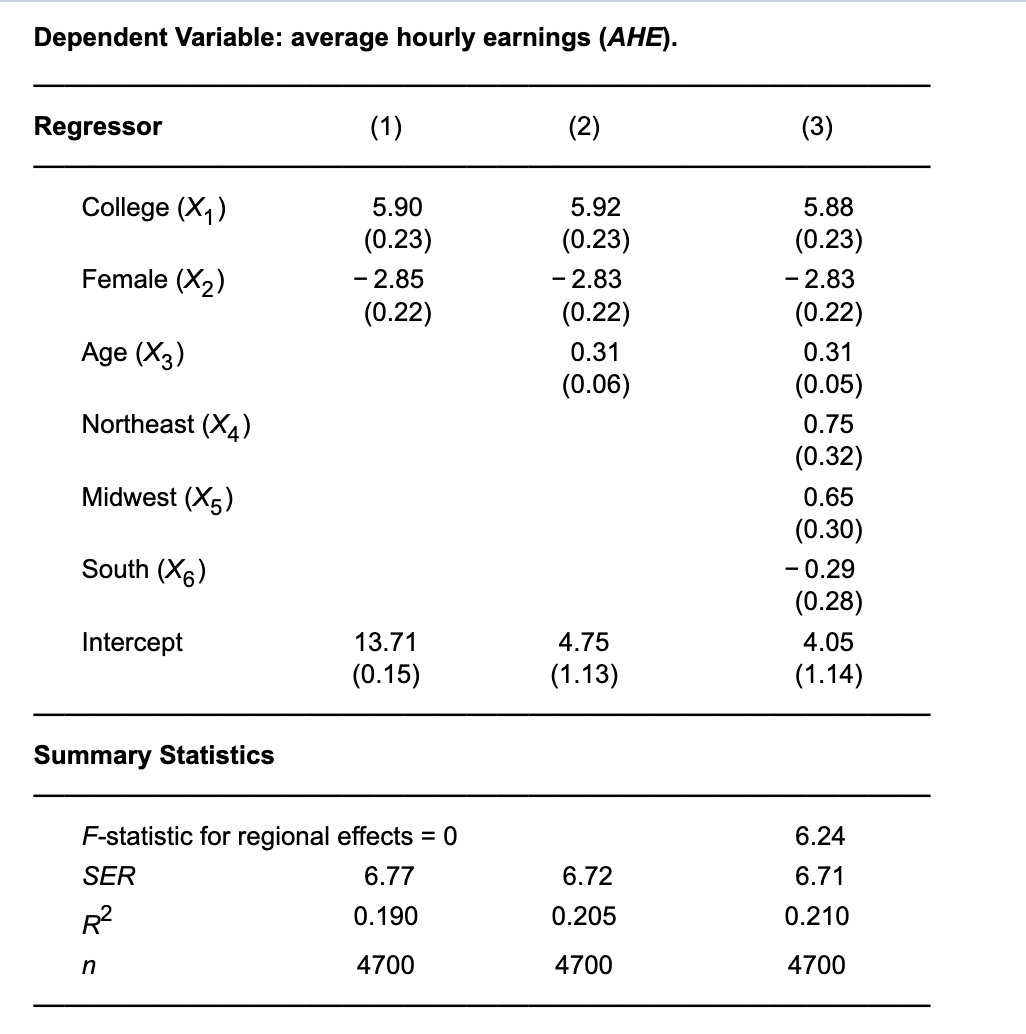
\includegraphics[scale=0.5]{materials/sw7-3.png}


\begin{longtable}[]{@{}ll@{}}
\toprule
Variable & Definition \\
\midrule
\endhead
AHE & average hourly earnings (in 2005 dollars) \\
College & 1 if college, 0 if high school \\
Female & 1 if female, 0 if male \\
Age & age (in years) \\
Ntheast & 1 if Region = Northeast, 0 otherwise \\
Midwest & 1 if Region = Midwest, 0 otherwise \\
South & 1 if Region = South, 0 otherwise \\
West & 1 if Region = West, 0 otherwise \\
\bottomrule
\end{longtable}

\begin{enumerate}
\def\labelenumi{\arabic{enumi}.}
\setcounter{enumi}{4}
\tightlist
\item
  Consider the regression results below and do the following:
\centering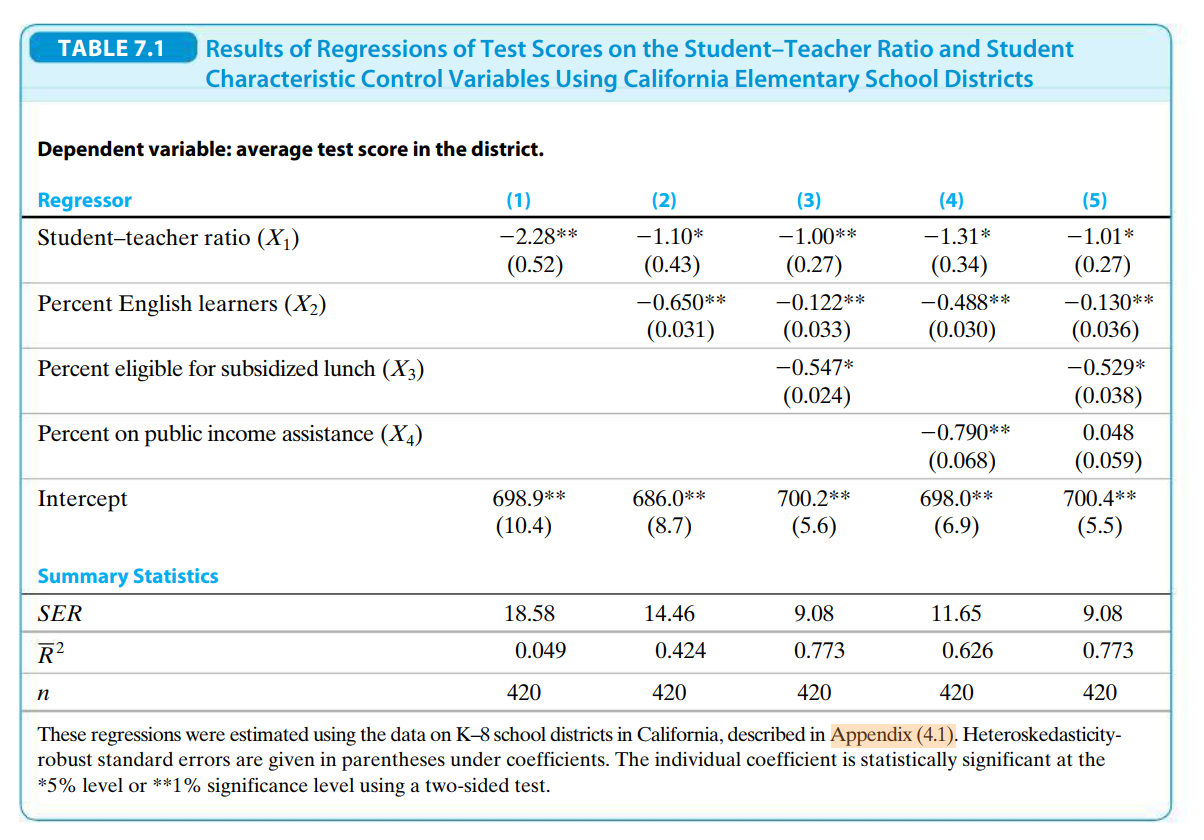
\includegraphics[scale=0.5]{materials/sw7-1.png}

  \begin{enumerate}
  \def\labelenumii{\alph{enumii}.}
  \tightlist
  \item
    Construct the \(R^2\) for each of the regressions
  \item
    Construct the homoskedasticity-only \(F\)-statistic for testing
    \(\beta_3 = \beta_4 = 0\) shown in column (5). Is the statistic
    significant at the 5\% level?
  \item
    Construct a 99\% confidence interval for \(\beta_1\) for the
    regression in column (5)
  \end{enumerate}
\end{enumerate}

\begin{enumerate}
\def\labelenumi{\arabic{enumi}.}
\setcounter{enumi}{5}
\tightlist
\item
  Download the dataset \href{https://ec200f21.netlify.app/assignment/materials/growth.dta}, which
  contains data on average growth rates from 1960 through 1995 for 65
  countries, along with variables that are potentially related to
  growth. You can download a detailed description of all variable names
  is available
  \href{https://www.princeton.edu/~mwatson/Stock-Watson_3u/Students/EE_Datasets/Growth_Description.pdf}{here}.
  For all questions, exclude Malta, which has an extremely high trade
  share. Estimate a regression of \texttt{growth} on
  \texttt{tradeshare}, \texttt{yearsschool}, \texttt{rev\_coups},
  \texttt{assassinations}, and \texttt{rgdp60}, with
  heteroskedasticity-robust standard errors.

  \begin{enumerate}
  \def\labelenumii{\alph{enumii}.}
  \tightlist
  \item
    What is the value of the coefficient on \texttt{rev\_coups}?
    Interpret the value of this coefficient. Is it large or small in a
    real-world sense?
  \item
    Use the regression to predict the average annual growth rate for a
    country has average valeus for all regressors.
  \item
    Construct a 90\% confidence interval for the coefficient on
    \texttt{tradeshare}. Is the coefficient statistically significant at
    the 10\% level? d.Test whether the political variables
    \texttt{rev\_coups} and \texttt{assassinations}, taken as a group,
    can be omitted from the regression. What is the p-value of the
    F-statistic?
  \end{enumerate}
\end{enumerate}

\end{document}
